% !TeX spellcheck = en_US
% Use only LaTeX2e, calling the article.cls class and 12-point type.

\documentclass[12pt]{article}

% Users of the {thebibliography} environment or BibTeX should use the
% scicite.sty package, downloadable from *Science* at
% www.sciencemag.org/about/authors/prep/TeX_help/ .
% This package should properly format in-text
% reference calls and reference-list numbers.

\usepackage{scicite}

% Use times if you have the font installed; otherwise, comment out the
% following line.

\usepackage{times}

% The preamble here sets up a lot of new/revised commands and
% environments.  It's annoying, but please do *not* try to strip these
% out into a separate .sty file (which could lead to the loss of some
% information when we convert the file to other formats).  Instead, keep
% them in the preamble of your main LaTeX source file.

\usepackage{graphicx}
\usepackage{csquotes}
\usepackage{hyperref}


% The following parameters seem to provide a reasonable page setup.

\topmargin 0.0cm
\oddsidemargin 0.2cm
\textwidth 16cm 
\textheight 21cm
\footskip 1.0cm


%The next command sets up an environment for the abstract to your paper.

\newenvironment{sciabstract}{%
\begin{quote} \bf}
{\end{quote}}


% If your reference list includes text notes as well as references,
% include the following line; otherwise, comment it out.

\renewcommand\refname{References and Notes}

% The following lines set up an environment for the last note in the
% reference list, which commonly includes acknowledgments of funding,
% help, etc.  It's intended for users of BibTeX or the {thebibliography}
% environment.  Users who are hand-coding their references at the end
% using a list environment such as {enumerate} can simply add another
% item at the end, and it will be numbered automatically.

\newcounter{lastnote}
\newenvironment{scilastnote}{%
\setcounter{lastnote}{\value{enumiv}}%
\addtocounter{lastnote}{+1}%
\begin{list}%
{\arabic{lastnote}.}
{\setlength{\leftmargin}{.22in}}
{\setlength{\labelsep}{.5em}}}
{\end{list}}


% Include your paper's title here

\title{LSTM Network for Song Genre Prediction based on Lyrics} 


% Place the author information here.  Please hand-code the contact
% information and notecalls; do *not* use \footnote commands.  Let the
% author contact information appear immediately below the author names
% as shown.  We would also prefer that you don't change the type-size
% settings shown here.

\author
{Andreas Rottach\
\\
\normalsize{CSI 52 - Artificial Intelligence}\\
\normalsize{An Introduction to Neural Networks and Deep Learning}\\
\normalsize{Continuing Studies, Stanford University}\\
\normalsize{Littlefield Center, 365 Lasuen St, Stanford, CA 94305, USA}\\
\\
\normalsize{E-mail: andreas@rottach.net}\\
\normalsize{SourceCode: \url{www.github.com/rottaca/LyricsClassifier}}
}

% Include the date command, but leave its argument blank.

\date{}



%%%%%%%%%%%%%%%%% END OF PREAMBLE %%%%%%%%%%%%%%%%



\begin{document} 

% Double-space the manuscript.

\baselineskip24pt

% Make the title.

\maketitle 



% Place your abstract within the special {sciabstract} environment.

\begin{sciabstract}
  During my internship at Mercedes-Benz R\&D in the Silicon Valley, I had the change to attend a machine learning class at Stanford University. For the final assignment we had the task to write a short science paper. Instead of summarizing an existing paper, I preferred doing my own small project. I implemented a machine learning solution, which is able to predict the genre of a song, based on parts of its lyrics. In this paper I will give a short summary about the implemented approach and its performance.
\end{sciabstract}



% In setting up this template for *Science* papers, we've used both
% the \section* command and the \paragraph* command for topical
% divisions.  Which you use will of course depend on the type of paper
% you're writing.  Review Articles tend to have displayed headings, for
% which \section* is more appropriate; Research Articles, when they have
% formal topical divisions at all, tend to signal them with bold text
% that runs into the paragraph, for which \paragraph* is the right
% choice.  Either way, use the asterisk (*) modifier, as shown, to
% suppress numbering.

\section{Introduction}

Processing of language and text is one of the big topics in modern machine learning and the use of neural networks gains more and more importance. The processing of text is not as easy as processing numerical input, which can be handled very well by all kinds of neural networks. Text, words or letters on the other hand have no implicit or explicit ordering compared and therefore mapping characters to their numerical counterparts with e.g. ASCII encoding usually doesn't give the desired result.
Over the years, several other approaches have been published in order to transform text into a more neural-network-friendly format. There are two common algorithms which transform words into vectors: word2vec \cite{goldberg2014word2vec} and glove \cite{pennington2014glove}. Both algorithms map words with similar meaning or co-occurrence to similar vectors in an N-dimensional vector space. By applying these word embeddings to text, processing of text is equivalent to processing a set of N-dimensional vectors.

Due to the temporal dependency between words in texts, LSTM\cite{gers1999learning} networks are usually the best machine learning architecture to choose. In contrast to basic recurrent networks, LSTM cells are better in extracting long-term temporal relationships in a sequence of inputs. For a more detailed explanation, please have a look at \cite{gers1999learning}.

\section{The Dataset}\label{sec:dataset}

In order to start the project, it was necessary to find a suitable dataset which contains an sufficient amount of song texts in an easy to parse data format. The used dataset was found at Kaggle: \blockquote{Kaggle is an online community of data scientists and machine learners, owned by Google LLC. Kaggle allows users to find and publish data sets, explore and build models ... 
}\footnote{\url{https://en.wikipedia.org/wiki/Kaggle} (03/02/2019)}. The used data set\footnote{\url{https://www.kaggle.com/gyani95/380000-lyrics-from-metrolyrics}} contains 380000 lyrics with additional metadata and is stored as csv table which allows easy import in python. The dataset contains mainly English songs but also Spanish, German and Chinese lyrics. Filtering out Chinese songs was easy (due to the different character set). All other lyrics for which the majority of words did not occur in the world embedding vocabulary (English words only) were removed as well. Originally, the dataset contains a varying number of songs per genre and therefore a fixed number of songs per genre was picked randomly in order to have an equal distribution over all genres.

After all preprocessing, the dataset contains approx. 50k lyrics equally distributed over 7 genres. The individual training samples are generated by moving a sliding window with fixed size (input sequence length) over each individual song text with a fixed stride of 2 words, in order to generate several position independent samples from a single song text. If a song contains less words than the window size requires or too may word were removed in the filter step, the song is not considered in the dataset. This is the case for 16521 songs. The genre names are converted to a 7 element one-hot vector encoding. For a window size of 50 , the final dataset is transformed into 3086740 (overlapping) sequences. Training and test data is split by a 9:1 ratio.

In addition to the dataset, glove word embeddings\footnote{\url{https://nlp.stanford.edu/projects/glove/}} were used. The embedding is pre-trained on a 6 billion word corpus with a vocabulary of 400k words, mapped to 100 dimensional vectors.

\section{The Algorithm}
As mentioned in the introduction, a word embedding (pretrained glove vectors) in combination with an LSTM network is used, to predict the genre of a song based on a fixed number of words (e.g. 50) from its lyrics. Figure \ref{fig:network1} shows the basic network architecture. The input (left) if fed into an embeddings layer. The transformed text is then fed into a (multi-layer) LSTM network which produces an M-dimensional output. This output is fed into a fully connected layer with a softmax activation function in order to generate prediction probabilities for each class. The final prediction is generated by selecting the output class with the highest probability.

\begin{figure}
	\centering
	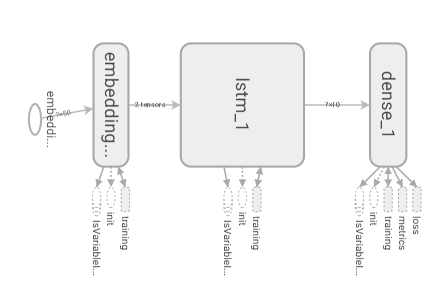
\includegraphics[width=0.7\textwidth]{img/network_simple.png}
	\caption{Neural network architecture (left to right): A world embeddings layer, an LSTM-Network and a fully connected sigmoid layer that generates the prediction.}
	\label{fig:network1}
\end{figure}

\section*{The Evaluation}
In order to evaluate this model, several combinations of parameters where tested. The set of parameters consists of the list shown below. Due to the limited time and computational power available, only some combinations of these parameters were tested. The ADAM optimizer was used to optimize the categorical cross entropy loss in order to training the network.

\begin{itemize}
	\item Number of LSTM layers in the network.
	\item Number of LSTM cells per layer.
	\item Input sequence length (number of words from a lyric).
	\item Use custom word embedding instead of pretrained one.
	\item Varying dimensionality of custom word embedding.
\end{itemize}

\paragraph*{Pretrained Word Embedding (Glove)}
The first tests were performed by using the pretrained glove word embedding with 100 dimensional vectors, trained on 6 billion tokens with a vocabulary of 400k different words. 

On one hand, using pretrained word embeddings is a good idea, because the training data covers many different topics and therefore the embedding has a quite good representation of relations between words in a generalized setup. This is beneficial for many different machine learning problems where it is hard to get enough training data for training a custom word embedding.

On the other hand, by simply using the word embedding as it is, only words existing in the vocabulary are considered and translated into numerical vectors. Unknown words require a special handling by e.g. checking if parts of words exist in the vocabulary or by setting the unknown words to a vector containing zeros only.

The problem with songs is, that they usually contain conversational language and words which can't be mapped to a vector that easily. The used dataset (after cleaning and filtering) has a vocabulary size of 116733 distinct words. Approximately 60k words can't be mapped to a glove vector (e.g. lyrics in a different languages) and therefore have to be mapped to zero. Training the network with these embedding gives the following result:

\begin{itemize}
	\item Changing the number of LSTM layers in the network has only minimal effect on the final performance, it just increases the number of parameters to optimize and slows down training.
	\item Changing the number of LSTM cells has the same effect as changing the number of layers. The training slows down with an increasing number of cells but the final performance stays the same.
	\item Varying the input sequence lengths from 50 to 100 words does slightly increase the final performance.
\end{itemize}

Random guessing results in a accuracy of 14.2 \% (with 8 output classes). This approach reaches an overall performance of 50\% accuracy after training as described in section \ref{sec:dataset}.

\paragraph*{Custom word embedding}
As described in the previous paragraph, using the pretrained word embedding has a few massive downsides in this use case due to the nature of song texts and their use of conversational language. Training a custom word embedding while training the network itself has the benefit of using all available words as actual input. This approach drastically increases training time but on the other hand, it allows the network to find a more suitable vector representation that simplifies the subsequent network training itself. This can also increase the importance of special words that might only occur in e.g. hip-hop songs.

In initial tests, the word embedding dimensionality was set to 64 but later reduced to 32 due to the limited number of words and the very small use case, which resulted in very similar performance but drastically increased training time. The LSTM layer size was set to 10 and 20 cells which was already good enough to result in acceptable performance. The sequence length was set to 50 words. Training a custom word embedding caused massive over fitting on the validation dataset due to the increased model complexity and the drastically increased number of free parameters.

\paragraph*{Final results}
Figure \ref{fig:results} shows the training results for a subset of all tested parameters. In general, the models with a custom trained word embedding have a slightly higher accuracy compared to the models based on the pretrained word embedding. The best performing model reaches an accuracy of 97\% on the training dataset and 56\% on the validation dataset with 20 LSTM cells, a custom word embedding with 32 dimensions and a history of 100 words. This is quite far from being perfect, but taking a closer look reveals that the correct classification is usually one of the top 3 most likely predictions. All custom word embeddings perform overfitting but this doesn't effect the categorical accuracy very much.

\begin{figure}[t!]
	\centering
	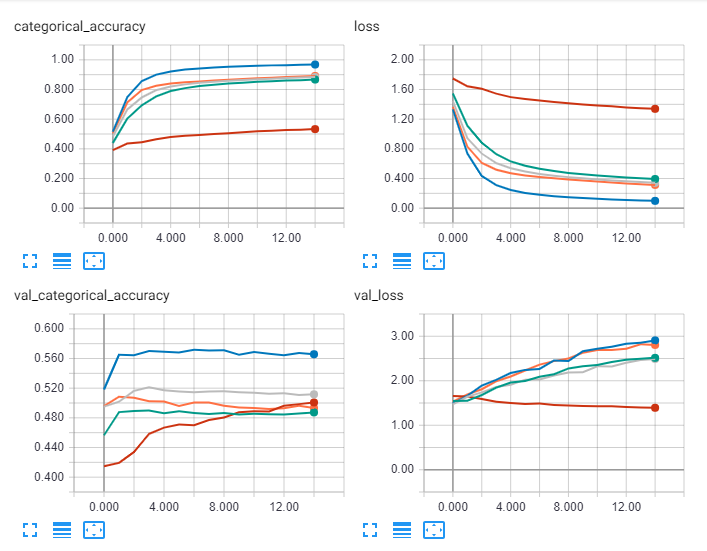
\includegraphics[width=0.9\textwidth]{img/results.png}
	\caption{Tensorboard plots for a subset of all trained networks. Blue: 20 LSTM cells, 32-dim custom embedding, 100 word history. Gray: 20 LSTM cells, 32-dim custom embedding, 50 word history, Orange: 40 LSTM cells, 32-dim custom embedding, 50 word history, Green: 10 LSTM cells, 32-dim custom embedding, 50 word history, Brown: 20 LSTM cells, 100-dim Glove embedding, 100 word history.}
	\label{fig:results}
\end{figure}

The performance of the network with highest accuracy is investigated a bit further. In order to have a closer look on the results, a per class accuracy for each individual song genre was computed. The results are show in figure \ref{tab:results}. This per class accuracy clearly shows, that the network is biased to Hip-Hop, Pop an Country songs whereas Jazz songs were never identified correctly. The reason for this behavior might be rooted in frequently occurring words in e.g. Hip-Hop songs. Another explanation is the fact that Hip-Hop songs usually have a higher word count compared to other genres which artificially biases the training dataset to more Hip-Hop samples (due to the sliding window approach as described in \ref{sec:dataset}). 

\begin{figure}
	\centering
\begin{tabular}{|c|c|}
	\hline 
	Class Name & Accuracy (\%) \\ 
	\hline 
	Hip-Hop & 85.6 \\ 
	\hline 
	Pop & 52.7 \\ 
	\hline 
	Country & 48.9 \\ 
	\hline 
	Rock & 10.0 \\ 
	\hline 
	Electronic & 9.4 \\ 
	\hline 
	R\&B & 8.3 \\ 
	\hline 
	Jazz & 0.0 \\ 
	\hline 
\end{tabular} 
\caption{This shows the per class accuracy for the best performing model, computed on the validation dataset. It is clearly visible that the network is biased to Hip-Hop songs.}
\label{tab:results}
\end{figure}

The best performing network produced the following output on the validation dataset (special characters removed, raw text only):

\begin{itemize}
	\item \textit{an accident one day that would chill the heart of any man it would teach them not to drink a drop while the steering wheel in their hand this awful accident occurred on the 20th day of may and caused two little children to be sleepin beneath the clay these two little kids walked side by side along the state highway their poor old mother she had died and their daddy had ran away as these two little children walked arm in arm how sad their hearts did feel when around the curb came a speeding car with a drunk }
	\begin{itemize}
		\item Top  predictions: Country (44.1\%), Rock (17.4\%), Metal (9.1\%)
		\item Label: Country
	\end{itemize}
	\item \textit{of perilous buried to remain among the vanquished there lies a key for which you must retrieve but once within your soul belongs to fire illusive concepts attempts un obtained those who before you became the detained within the gates you seek fading light buried in darkness your sense filled with fright within the gates you will tempt fate you must beware you are the chosen one dark ruler only son the power you posses is now the final chance within the gates you will tempt fate you must beware theme solo theme walk towards the fading light alone wide }
	\begin{itemize}
		\item Top  predictions: Metal (71.7\%), Rock (11.5\%), Electronic (4.3\%)
		\item Label: Metal
	\end{itemize}
	\item \textit{for the hungry and underprivileged something different from these hollow and grunting niggas this is business strictly step to my business is risky specially when you as bitch as missy back to back lp that sound the same i surround the game with a four pounded brainstorm to make niggas dance in the rain scared to take a chance in the game used to break dance it a shame what money do to a nigga brain if he lose his soul what did a nigga gain doin it doin it i am doin it c o double m o to}
	\begin{itemize}
		\item Top  predictions: Hip-Hop (97.4\%), Metal (1.1\%), Rock (0.5\%)
		\item Label: Hip-Hop
	\end{itemize}
	\item \textit{me mind when i looked behind no bundle could i find upon me stick a wobblin enquiring for the rogue they said me connaught brogue wasnt much in vogue on the rocky road to dublin one two three four five hunt the hare and turn her down the rocky road all the way to dublin whack follol de rah from there i got away me spirits never falling landed on the quay just as the ship was sailing the captain at me roared said that no room had he when i jumped aboard a cabin found for paddy down among}
	\begin{itemize}
		\item Top  predictions: Country (37.5\%), Rock (18.6\%), Pop (10.3\%)
		\item Label: Pop
	\end{itemize}
\end{itemize}

% Your references go at the end of the main text, and before the
% figures.  For this document we've used BibTeX, the .bib file
% scibib.bib, and the .bst file Science.bst.  The package scicite.sty
% was included to format the reference numbers according to *Science*
% style.

\section{Summary}

As shown in the previous chapters, the implemented solution is able to reach an accuracy between 50 and 60 percent which is far better than random guessing with 7 options (14 percent). Nevertheless, the proposed solution has short comings and is far from being perfect. Issues arise from the usage of conversational language as well mixed languages in the training dataset. Issues with the pretrained word embedding can also be reduced by searching for sub-words in the vocabulary and building embeddings vectors based on these sub-words. By doing so, more words can be used for the actual training of the network.
The performance might also be improved by training a custom word embedding on a larger dataset of songs and it might be possible to apply other approaches like convolutional neural networks to solve this task. Nevertheless, the proposed solution gives acceptable results for such a simple architecture.

\bibliography{scibib}
\bibliographystyle{acm}


\end{document}
 



















